%% For double-blind review submission, w/o CCS and ACM Reference (max submission space)
\documentclass[sigplan,10pt,review]{acmart}\settopmatter{printfolios=true,printccs=false,printacmref=false}
%% For double-blind review submission, w/ CCS and ACM Reference
%\documentclass[sigplan,10pt,review,anonymous]{acmart}\settopmatter{printfolios=true}
%% For single-blind review submission, w/o CCS and ACM Reference (max submission space)
%\documentclass[sigplan,10pt,review]{acmart}\settopmatter{printfolios=true,printccs=false,printacmref=false}
%% For single-blind review submission, w/ CCS and ACM Reference
%\documentclass[sigplan,10pt,review]{acmart}\settopmatter{printfolios=true}
%% For final camera-ready submission, w/ required CCS and ACM Reference
%\documentclass[sigplan,10pt]{acmart}\settopmatter{}


%% Conference information
%% Supplied to authors by publisher for camera-ready submission;
%% use defaults for review submission.
\acmConference[PL'17]{ACM SIGPLAN Conference on Programming Languages}{January 01--03, 2017}{New York, NY, USA}
\acmYear{2017}
\acmISBN{} % \acmISBN{978-x-xxxx-xxxx-x/YY/MM}
\acmDOI{} % \acmDOI{10.1145/nnnnnnn.nnnnnnn}
\startPage{1}

%% Copyright information
%% Supplied to authors (based on authors' rights management selection;
%% see authors.acm.org) by publisher for camera-ready submission;
%% use 'none' for review submission.
\setcopyright{none}
%\setcopyright{acmcopyright}
%\setcopyright{acmlicensed}
%\setcopyright{rightsretained}
%\copyrightyear{2017}           %% If different from \acmYear

%% Bibliography style
\bibliographystyle{ACM-Reference-Format}
%% Citation style
%\citestyle{acmauthoryear}  %% For author/year citations
%\citestyle{acmnumeric}     %% For numeric citations
%\setcitestyle{nosort}      %% With 'acmnumeric', to disable automatic
                            %% sorting of references within a single citation;
                            %% e.g., \cite{Smith99,Carpenter05,Baker12}
                            %% rendered as [14,5,2] rather than [2,5,14].
%\setcitesyle{nocompress}   %% With 'acmnumeric', to disable automatic
                            %% compression of sequential references within a
                            %% single citation;
                            %% e.g., \cite{Baker12,Baker14,Baker16}
                            %% rendered as [2,3,4] rather than [2-4].


%%%%%%%%%%%%%%%%%%%%%%%%%%%%%%%%%%%%%%%%%%%%%%%%%%%%%%%%%%%%%%%%%%%%%%
%% Note: Authors migrating a paper from traditional SIGPLAN
%% proceedings format to PACMPL format must update the
%% '\documentclass' and topmatter commands above; see
%% 'acmart-pacmpl-template.tex'.
%%%%%%%%%%%%%%%%%%%%%%%%%%%%%%%%%%%%%%%%%%%%%%%%%%%%%%%%%%%%%%%%%%%%%%


%% Some recommended packages.
\usepackage{booktabs}   %% For formal tables:
                        %% http://ctan.org/pkg/booktabs
\usepackage{subcaption} %% For complex figures with subfigures/subcaptions
                        %% http://ctan.org/pkg/subcaption

\usepackage{graphicx}
\usepackage{graphics}
\usepackage{amsmath,amssymb, amsfonts, mathtools}
\usepackage{isabelle,isabellesym}

\newcommand{\defeq}{\mathrel{\stackrel{\mbox{\tiny \it def}}{=}}}
\newcommand{\sconj}{\wedge^*}
\newcommand{\coloncolon}{\mathrel{::}}
\newcommand{\pvalid}[3]{\models\{#1\}\:#2\:\{#3\}}
\newcommand{\tvalid}[3]{\models[#1]\:#2\:[#3]}
\newcommand{\ttrip}[5]{\mathit{#1} \vdash_{\mathrm{#2}}[#3]\:#4\:[#5]}
\newcommand{\xnext}{\mathit{next}}
\newcommand{\code}[1]{\mathit{code}(#1)}
\newcommand{\cont}{\mathit{continuing}}
\newcommand{\ncont}{\mathit{not\_continuing}}
\newcommand{\instr}[1]{\mathtt{#1}}
\newcommand{\Rule}[2]{\begin{array}{c}#1\\\hline\noalign{\smallskip}#2\end{array}}
%\newcommand{\Rule}[2]{\dfrac{#1}{#2}}


%%%%%%%%%%%%%%%%%%
\newcommand{\sid}[1]{\textit{\textbf{#1 [sid]}}}







\begin{document}

%% Title information
\title[Towards Verifying Ethereum Smart Contracts]{Towards Verifying Ethereum Smart Contract Bytecode in Isabelle/HOL}         %% [Short Title] is optional;
                                        %% when present, will be used in
                                        %% header instead of Full Title.
%\titlenote{with title note}             %% \titlenote is optional;
                                        %% can be repeated if necessary;
                                        %% contents suppressed with 'anonymous'
%\subtitle{Subtitle}                     %% \subtitle is optional
%\subtitlenote{with subtitle note}       %% \subtitlenote is optional;
                                        %% can be repeated if necessary;
                                        %% contents suppressed with 'anonymous'


%% Author information
%% Contents and number of authors suppressed with 'anonymous'.
%% Each author should be introduced by \author, followed by
%% \authornote (optional), \orcid (optional), \affiliation, and
%% \email.
%% An author may have multiple affiliations and/or emails; repeat the
%% appropriate command.
%% Many elements are not rendered, but should be provided for metadata
%% extraction tools.

%% Authors with single affiliation.

%% AUTHORS APPEAR IN ALPHABETIC ORDER

\author{Sidney Amani}
%\authornote{with author1 note}          %% \authornote is optional;
                                        %% can be repeated if necessary
%\orcid{nnnn-nnnn-nnnn-nnnn}             %% \orcid is optional
\affiliation{
%  \position{Position1}
  \department{Data61}              %% \department is recommended
  \institution{CSIRO}            %% \institution is required
%  \streetaddress{Street1 Address1}
%  \city{City1}
  \state{NSW}
%  \postcode{Post-Code1}
  \country{Australia}                    %% \country is recommended
}
\email{Sidney.Amani@data61.csiro.au}          %% \email is recommended

\author{Myriam B\'egel}
\authornote{work done while at Data61, CSIRO}          %% \authornote is optional;
                                        %% can be repeated if necessary
%\orcid{nnnn-nnnn-nnnn-nnnn}             %% \orcid is optional
\affiliation{
%  \position{Position1}
%  \department{Department1}              %% \department is recommended
  \institution{\'Ecole Normale Sup\'erieure Paris-Saclay}            %% \institution is required
%  \streetaddress{Street1 Address1}
%  \city{City1}
%  \state{State1}
%  \postcode{Post-Code1}
  \country{France}                    %% \country is recommended
}
\email{Myriam.Begel@ens-paris-saclay.fr}          %% \email is recommended


\author{Maksym Bortin}
%\authornote{with author1 note}          %% \authornote is optional;
                                        %% can be repeated if necessary
%\orcid{nnnn-nnnn-nnnn-nnnn}             %% \orcid is optional
\affiliation{
%  \position{Position1}
  \department{Data61}              %% \department is recommended
  \institution{CSIRO}            %% \institution is required
%  \streetaddress{Street1 Address1}
%  \city{City1}
  \state{NSW}
%  \postcode{Post-Code1}
  \country{Australia}                    %% \country is recommended
}
\email{Maksym.Bortin@data61.csiro.au}          %% \email is recommended

\author{Mark Staples}
%\authornote{with author1 note}          %% \authornote is optional;
                                        %% can be repeated if necessary
%\orcid{nnnn-nnnn-nnnn-nnnn}             %% \orcid is optional
\affiliation{
%  \position{Position1}
  \department{Data61}              %% \department is recommended
  \institution{CSIRO}            %% \institution is required
%  \streetaddress{Street1 Address1}
%  \city{City1}
  \state{NSW}
%  \postcode{Post-Code1}
  \country{Australia}                    %% \country is recommended
}
\email{Mark.Staples@data61.csiro.au}          %% \email is recommended

%% Abstract
%% Note: \begin{abstract}...\end{abstract} environment must come
%% before \maketitle command
\begin{abstract}
Blockchain technology has increasing attention in research and across many industries.
The Ethereum block-chain offers \emph{smart contracts}, which are small programs defined,
executed, and recorded as transactions in the blockchain transaction history.
These smart contracts run on the Ethereum virtual machine (EVM) and can be used to encode
agreements, transfer assets, and enforce integrity conditions in relationships between parties.
Smart contracts can carry financial value, and are increasingly
used for safety-, security-, or mission-critical purposes.
Errors in smart contracts have and will lead to loss or harm.
Formal verification can provide the highest level of confidence about the
correct behaviour of smart contracts.
In this paper we extend an existing EVM formalisation~\cite{Yoichi} in Isabelle/HOL by a sound
program logic at the level of bytecode.
We structure and reason about bytecode sequences into graphs of basic blocks of straight-line
code.
This abstraction is a step towards control of the cost and complexity of formal verification
of EVM smart contracts.
\end{abstract}


%% 2012 ACM Computing Classification System (CSS) concepts
%% Generate at 'http://dl.acm.org/ccs/ccs.cfm'.
\begin{CCSXML}
<ccs2012>
<concept>
<concept_id>10011007.10011006.10011008</concept_id>
<concept_desc>Software and its engineering~General programming languages</concept_desc>
<concept_significance>500</concept_significance>
</concept>
<concept>
<concept_id>10003456.10003457.10003521.10003525</concept_id>
<concept_desc>Social and professional topics~History of programming languages</concept_desc>
<concept_significance>300</concept_significance>
</concept>
</ccs2012>
\end{CCSXML}

\ccsdesc[500]{Software and its engineering~General programming languages}
\ccsdesc[300]{Social and professional topics~History of programming languages}
%% End of generated code


%% Keywords
%% comma separated list
\keywords{formal verification, blockchain, smart contracts, Ethereum, Isabelle/HOL}  %% \keywords are mandatory in final camera-ready submission


%% \maketitle
%% Note: \maketitle command must come after title commands, author
%% commands, abstract environment, Computing Classification System
%% environment and commands, and keywords command.
\maketitle


\section{Introduction}
\label{sec:intro}
Blockchain technology emerged to support financial transactions in the Bitcoin system, but has become
increasingly important in many industries, with potential use in legal, medical, and
supply chain industries.
The Ethereum blockchain provides a general-purpose computational mechanism called \emph{smart contracts}.
These are programs that run on the Ethereum virtual machine~\cite{wood2014ethereum} (EVM), and
are recorded in the blockchain history.  They can be used to encode or execute agreements between parties.
For example, a party invoking a smart contract could cause digital currency to be transferred to another
party, or could record a state change which makes the other party eligible to invoke other transactions.
Smart contracts provide new ways to implement multi-party relationships within blockchain-based applications.
In addition to the direct financial value in these applications, blockchains are increasingly being
used for safety-critical applications such for pharmaceutical supply chains, or for mission-critical
application such as in electrical power grids.
We must know that smart contract implementations do not violate critical requirements, and
formal modelling and verification can be applied in this context.
%
To address these questions we seek:
\begin{itemize}
\item[(i)] a trustworthy logical framework capable of expressing complex safety and security
   requirements; 
\item[(ii)] a valid formal model of the EVM within the framework; 
\item[(iii)] a sound program logic defined within the framework able to
reason about properties of smart contracts. 
\end{itemize}
In our setting, we use the logical framework Isabelle/HOL, and an existing EVM formal
model~\cite{Yoichi}.
Thus, our remaining goal is a sound program logic.  In this paper we propose such a logic for EVM bytecode. 
We target unstructured bytecode rather than a high-level programming language for several reasons.
Firstly, our approach is independent of high-level languages (e.g.\ Solidity) and their compilers, which
makes our work more general and significantly less reliant
on the correctness of higher-level tools.
Secondly, bytecode is the actual programming language of Ethereum as all smart contracts appear only
in this form on the blockchain.
Thus we target EVM bytecode, despite the necessity for us to restore structures (such as conditionals)
that we might take for granted in higher-level languages.
We describe our approach for this in the remainder of the paper. 

The main contributions of the paper are:
\begin{itemize}
\item[(i)] an extension to the EVM formalisation~\cite{Yoichi} in the Isabelle/HOL theorem prover,
           covering smart contract correctness properties, and which gives a separate universal
           treatment of termination based on Ethereum's concept of execution `gas';
\item[(ii)] a sound program logic to verify smart contracts at the bytecode level; and
\item[(iii)] Isabelle tactics to support automated generation of verification
            conditions using the rules of the logic.
\end{itemize}
         
The paper is structured as follows. Sections~\ref{sec:bg} and \ref{sec:rwork} describe background
and the related work. Section~\ref{sec:corr} describes correctness properties in a pre/postcondition
style for EVM bytecode programs. Section~\ref{sec:logic} is devoted to our program logic, 
%i.e. rules for generation of verification conditions out of a contract, 
and Section~\ref{sec:sound} shows the soundness of the logic
w.r.t. the correctness property. Section~\ref{sec:auto} outlines how we automate generation of verification
conditions using Isabelle tactics. Section~\ref{sec:case} presents a case-study deploying our framework in 
real bytecode verification, and
Section~\ref{sec:concl} summarises the results and gives an outlook for future work.
%
\section{Background} 
\label{sec:bg}
The EVM is described in the Ethereum `Yellow Paper'~\cite{wood2014ethereum}.
This provides a clear foundation not only for its implementation, but also for its formalisation in logic.
One such formalisation has been provided~\cite{Yoichi} using the `meta-tool' \emph{Lem}~\cite{DBLP:conf/icfp/MulliganOGRS14}.
Lem supports a variety of theorem provers including Isabelle/HOL.
\emph{Isabelle}~\cite{Nipkow_PW:Isabelle} is a logical framework and interactive generic theorem prover.
Isabelle/HOL encodes higher-order logic and is the most important and most developed logic in Isabelle.
Isabelle's LCF-style architecture,
based on a small (meta)-logical inference kernel, provides very high confidence about its sound
implementation as a theorem prover.
 
The EVM formalisation needs to be validated to provide confidence that the formal model
and EVM implementations coincide. To this end, a validation test suite accompanies
the model in Lem. Using this, EVM implementations and OCaml code generated by Lem from the EVM
formal model are both applied to a large collection of contracts, cross-checking their outputs.  

We entirely focus on the EVM model in Isabelle/HOL, so additionally run the test suite 
on OCaml code generated by Isabelle. This our `double-validation' 
process as outlined in Figure~\ref{fig:valid}.          
\begin{figure}[htbp]
\centering
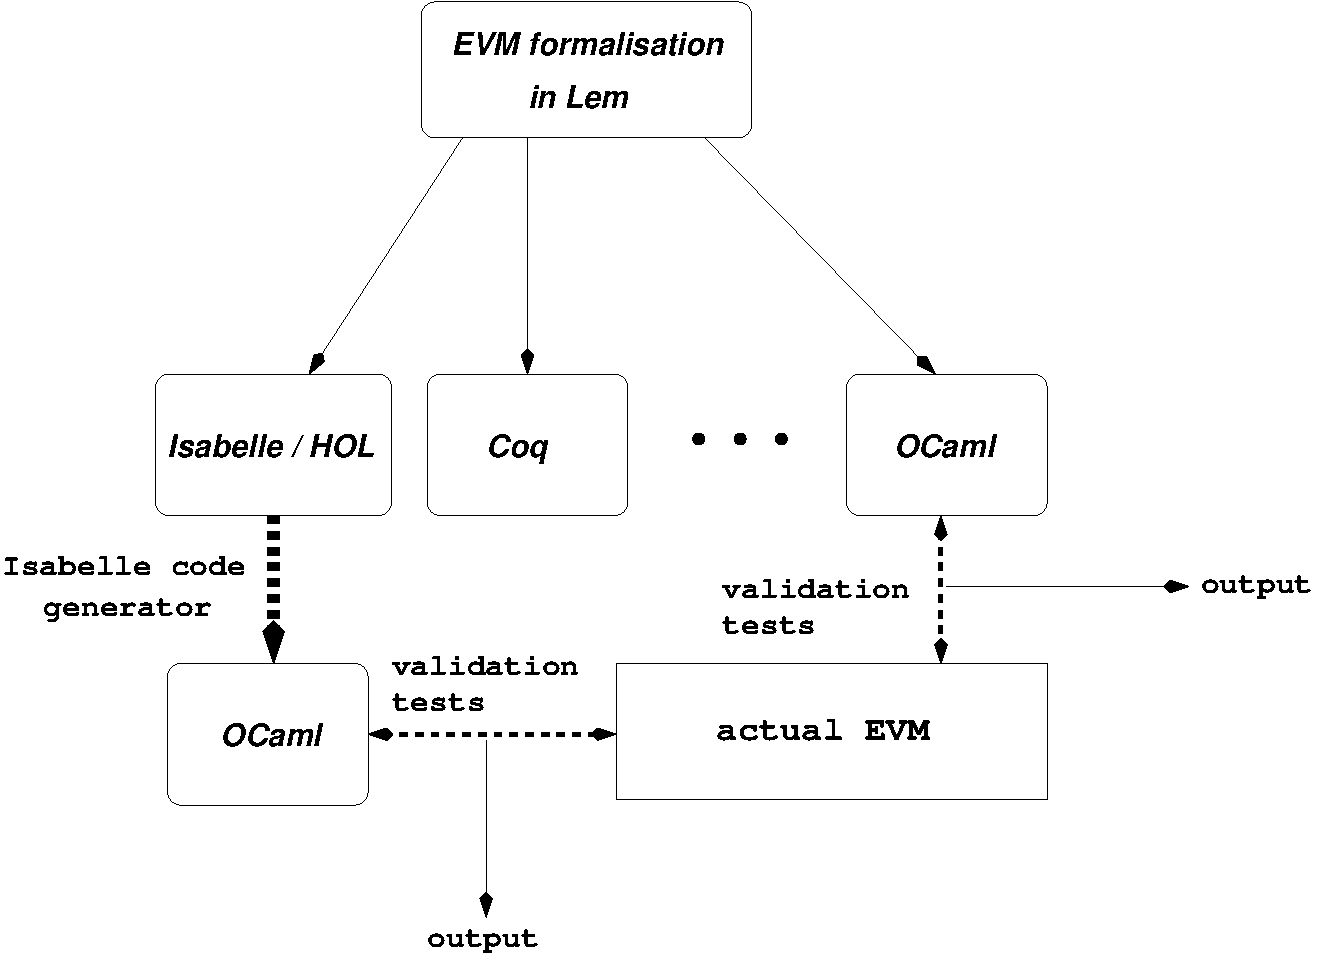
\includegraphics[height=5.5cm, width=7.5cm]{images/evm_lem}    
        \caption{Validation of EVM models}
\label{fig:valid}
\end{figure}
The use of the test suite from Isabelle has required certain efforts, mainly because 
of different representations of machine words. OCaml code from Lem uses efficient native modules,
whereas the Isabelle side invokes a formally-verified theory of machine words.
Because of this, our suite needs much more time to pass the tests.
Nonetheless, we gain a complementary indication that all three models of EVM follow the specification
and behave equally.    
%
\section{Related Work}
\label{sec:rwork}


\sid{XCAP, Chlipala's bedrock, KEVM?}
As a consequence of the fact that smart contracts are critical under many aspects, a notable amount of
approaches and tools for their analysis has already been proposed 
(\cite{Bhargavan:2016:FVS:2993600.2993611}, \cite{securify}, \cite{openzeppelin} to name a few).
 
The major trend is to apply various kinds of static analysis not only at the level of structured contract
languages (e.g. Solidity's Why3 backend~\cite{filliatre2013why3}) but also at the bytecode level~\cite{Msuiche_17,securify}. 
%However, most tools do not provide a lot of insight into internal details.
%
The obvious advantage of static analysis approaches is that full automation can be achieved for 
contract properties that can be confirmed statically, e.g. certain orders of transactions \cite{securify} 
 
Our approach is general as we aim to specify and verify contract properties in pre/postcondition
style where the conditions can comprise any higher-order logic formula describing an EVM state. 
For that reason, the degree of automation is basically limited in our case such that the user will need to interact 
with the proof system in most cases to discharge elaborated claims. 

In~\cite{Bhargavan:2016:FVS:2993600.2993611}, a technique using an intermediate functional language
called $F^*$, which is more amenable to verification, has been proposed. 
It provides not only translation of a subset of Solidity programs 
to $F^*$, but also decompilation of EVM bytecode to $F^*$ as well. This use of decompilation makes
the approach similar to ours, since our program logic, in fact, resembles decompilation.
As we will show in the following sections, in the first step we split bytecode program into blocks without jumps,  
whereas the actual jump destinations are determined dynamically `on-the-fly' by application of logic rules.
By contrast, \cite{Bhargavan:2016:FVS:2993600.2993611} performs static stack analysis to this end.
However, a more striking difference is that our approach is homogeneous since basically each and every step of our whole verification process 
is performed and justified within a single, trusted logical framework without any translations to or from other formalisms.
As already mentioned, such translations must be either assumed to behave correctly in some sense or 
formally modelled and verified,
whereas we aimed to avoid both of these options. 
%   
\section{Total Correctness of EVM Bytecode Programs}
\label{sec:corr}
In his PhD thesis~\cite{DBLP:phd/ethos/Myreen09}, Myreen introduced a general 
method of formal 
machine code verification with a particular application to ARM. In this section we show how
this general method can be adapted to EVM, taking however additional accounts of its specific properties rooted in the 
gas consumption.
 
In the general model, a state carries all the information needed to execute a program, including
instructions (with respective reference numbers) constituting the program itself, a program counter that
refers to the current instruction, a stack and so on. All these elements are treated uniformly 
as sets of so-called \emph{state elements}
and separated in a state using separation logic conjuncts $\sconj$~\cite{Reynolds_02}.  
Then a single machine step can be captured by a function $\xnext$ that 
takes the current instruction and transforms the state in accordance with the instructions
specified behaviour. Of course, $\xnext$ might not always be able to pick an instruction
as an execution can have terminated properly or with an exception. This is indicated within a state
by the $\ncont$ flag, which is just an abbreviation for the state element 
$\mathit{ContinuingElm}\:False$. If $\ncont$ is present in a state, $\xnext$
leaves the state unchanged.   
   
An input/output property of a program $c$ is captured by a triple
$\pvalid{P}{c}{Q}$ which is true iff for any state $s$ and frame $F$ such that
$(P \sconj \code{c} \sconj F)\: s$ holds, there exists a natural number $k$ such that 
$(Q \sconj \code{c} \sconj F)\: \xnext^k(s)$ holds. 
%The frame is used to accomodate an invariant part of a state, 
Keeping frame $F$ will allow us to reason about parts of the state locally using \emph{frame rule}(cf.~\cite{Reynolds_02}),
whereas $\xnext^k$ as usual denotes the $k$-times iteration of $\xnext$.
Such triples $\pvalid{P}{c}{Q}$ are highly generic and we cannot conclude much from many of these, except that
under given preconditions the program $c$ will pass a state satisfying $Q$. This changes immediately in cases when $Q$ is of
the form $\ncont \sconj Q'$, now stating that $c$ has reached a terminating state satisfying $Q'$.
Hence, showing $\pvalid{P}{c}{\ncont \sconj Q'}$ amounts to showing termination of the program $c$ in
a $Q'$-state.

\sid{Clarify purpose of gas comsumption in the Ethereum protocol in general and
how it works w.r.t. the EVM.}
This general approach seamlessly applies to the specific case of EVM bytecode. However,
due to the fact that EVM serves a blockchain, it exhibits a specific property that we have observed and exploit below, 
simplifying the method. 
So, by design, execution of each EVM instruction requires some respective positive amount of gas which
is subtracted after the execution from the overall gas amount assigned to this contract. 
Otherwise, the contract cannot proceed and exits with an exception.  
This property gives us a termination order, such that in this context we have the function $\xnext^*$ which 
consequently assigns to each state the terminal element from the reflexive-transitive closure of $\xnext$. 
The essential property of $\xnext^*$ is that for any state $s$ there exists $k \geq 0$ such that
\begin{itemize}
\item[(i)] $\xnext^*(s) = \xnext^k(s)$
\item[(ii)] $\xnext^l(s)$ can continue for any $l$ such that $0 \le l < k$
\item[(iii)] $\xnext^l(s)$ cannot continue for any $l \ge k$.
\end{itemize}
In other words, $\xnext^*(s) = \xnext^k(s)$ where $k$ is the least number such that
$\xnext^k(s)$ reaches a state with $\ncont$. 

Now, regarding the contract correctness, we strengthen $\pvalid{P}{c}{Q}$ to 
a total correctness property $\tvalid{P}{c}{Q}$ which is consequently true iff
for any state $s$ and frame $F$ 
$(P \sconj \code{c} \sconj F)\: s$ implies $(Q \sconj \code{c} \sconj F)\: \xnext^*(s)$. 
To sum up, what we achieved so far is to factor out the termination part which we have 
shown \emph{once and for all} contracts, thus removing this obligation from the verification
process completely. In the next section we will present our program logic handling EVM bytecode, 
which (based on soundness presented in Section~\ref{sec:sound}) will give us 
a sound device to derive verification conditions for contract properties of the form $\tvalid{P}{c}{Q}$.   
%       
\section{Program Logic}
\label{sec:logic}
A Hoare-style program logic comprises a collection of rules that allow us to derive semantic properties 
of compound programs from properties of its parts. In case of structured languages 
we usually have, for instance, a rule telling us that a program \textbf{if} $C$ \textbf{then} $p_1$ \textbf{else} $p_2$
exhibits a certain input/output behaviour if $p_1$ and $p_2$ do so, however, with the additional precondition $C$ 
available for $p_1$ and $\neg C$ -- for $p_2$. The situation is not that simple when we have to deal with mainly
unstructured programs like EVM bytecode in our case. For example, such conditional compound constructs as above
appear merely as instructions to make jumps to other program parts. Since a bytecode program comprises
a list of instructions, a rule might handle the head instruction and proceed to the tail of 
the list, but would need to make exceptions when the head instruction is a jump, because then
we cannot simply proceed with the tail. Although such treatment is in principle possible,
there are more sophisticated decompilation techniques available, such as extraction of 
\emph{Control Flow Graphs} (CFG), in particular applied to the Java Virtual Machine (JVM) code~\cite{zhao99}.
The aim of CFG extraction is to split a program into \emph{basic blocks}, i.e. sequences of
instructions without jumps, and connect them
using edges corresponding to jumps. Obviously, the essential property of basic blocks is that
control flow always enters it at its first instruction and leaves only after the last one
has been executed.

However, CFG extraction for JVM cannot be easily adapted to our EVM context, because JVM jump
instructions carry their respective target address statically, whereas in EVM jump destinations
must be obtained from the stack, i.e. dynamically. For that reason, our bytecode preprocessing
currently addresses basic block extraction only.  
%       
\subsection{Extraction of Basic Blocks}
We divide instructions into three groups:
\begin{itemize}
\item[(i)] $\instr{JUMPDEST}$ -- indicates a jump destination and hence beginning of a
                                 basic block;
\item[(ii)] $\instr{JUMP}$, $\instr{JUMPI}$, $\instr{UNKNOWN}$ and all of so-called 
            \emph{Misc}-instructions\footnote{RETURN, STOP, SUICIDE, CREATE, CALL, CALLCODE, DELEGATECALL} --
            indicate the end of a basic block ($\instr{UNKNOWN}$ and Misc-instructions interrupt program execution); 
\item[(iii)] all remaining instructions that form the contents of basic blocks.
\end{itemize}  
Furthermore, we classify basic blocks by means of the following four types:
\begin{itemize}
\item[(i)] \textit{Terminal} -- if the last instruction of the block interrups execution;
\item[(ii)] \textit{Jump} -- if the last instruction is $\instr{JUMP}$;
\item[(iii)] \textit{Jumpi} -- if the last instruction is $\instr{JUMPI}$;
\item[(iv)] \textit{Next} -- otherwise, i.e. when control passes from the last instruction of the block
                             to the instruction with the successor address.                         
\end{itemize} 
Figure~\ref{fig:basicblocks} illustrates how we split EVM bytecode into basic blocks of different
types, thereby indexing the blocks with addresses of their head instructions as well as removing all jump 
instructions from their actual contents. The entire extraction process is captured in Isabelle
by means of a function $\mathit{build\_blocks}$ which maps a list of instructions to a list of tuples $(i, \mathit{xs}, t)$, 
where $i$ is the block index, $\mathit{xs}$ -- the list of instructions of the block, and $t$ -- the type of
the block. 
%Moreover, we keep the order of blocks such that we can refer to the block where   
\begin{figure}
\center
\begin{tabular}{c r l c}
                block index & index & instruction & block type\\
                        \hline
                &       0       &       $\instr{OR}$&\\
                &       1       &       $\instr{ADD}$&\\
                {0}&    2       &       $\instr{SWAP1}$&  \textit{Next}\\
                        \hline
                &       3       &       $\instr{JUMPDEST}$&\\
                &       4       &       $\instr{MLOAD}$&\\
                &       5       &       $\instr{POP}$&\\
                {3}&    \textcolor{gray}{6}     &       {\color{gray}$\instr{JUMP}$}& \textit{Jump}\\
                        \hline
                &       7       &       $\instr{DUP3}$&\\
                &       8       &       $\instr{PUSH 0}$&\\
                &       10      &       $\instr{ISZERO}$&\\
                {7}&    \textcolor{gray}{11}    &       {\color{gray}$\instr{JUMPI}$}& \textit{Jumpi}\\
                        \hline
                &       12      &       $\instr{POP}$&\\
                {12}&   13      &       $\instr{RETURN}$& \textit{Terminal}\\
                        \hline
        \end{tabular}
\caption{A program splitted into basic blocks, where grey instructions appear in the original 
         code but are removed from the list of instructions of their block.}
\label{fig:basicblocks}
\end{figure}

\section{Soundness}
\label{sec:sound}


\section{Proof Automation}
\label{sec:auto}


\section{Case-study}
\label{sec:case}


\section{Conclusions and Future Work}
\label{sec:concl}

%% Acknowledgments
%\begin{acks}                            %% acks environment is optional
                                        %% contents suppressed with 'anonymous'
  %% Commands \grantsponsor{<sponsorID>}{<name>}{<url>} and
  %% \grantnum[<url>]{<sponsorID>}{<number>} should be used to
  %% acknowledge financial support and will be used by metadata
  %% extraction tools.
%  This material is based upon work supported by the
%  \grantsponsor{GS100000001}{National Science
%    Foundation}{http://dx.doi.org/10.13039/100000001} under Grant
%  No.~\grantnum{GS100000001}{nnnnnnn} and Grant
%  No.~\grantnum{GS100000001}{mmmmmmm}.  Any opinions, findings, and
%  conclusions or recommendations expressed in this material are those
%  of the author and do not necessarily reflect the views of the
%  National Science Foundation.
%\end{acks}


%% Bibliography
\bibliography{evm}


%% Appendix
%\appendix
%\section{Appendix}
%Text of appendix \ldots

\end{document}
